\documentclass[12pt,letterpaper]{article}

%Trennungsregeln etc.
\usepackage[english]{babel}

%Schriftart
%see http://www.tug.dk/FontCatalogue/ for more
%Ideen: baskervald
%for working: arev
\usepackage{baskervald}

%Sonderzeichenein-/ausgabe (http://tex.stackexchange.com/questions/44694/fontenc-vs-inputenc for questions)
\usepackage[utf8]{inputenc}
\usepackage[T1]{fontenc}

%Zeilenabstand, Optionen: singlespacing, onehalfspacing, doublespacing
\usepackage[onehalfspacing]{setspace}

%Seitenränder, hier oneside
\usepackage[left=2.5cm,right=2.5cm,top=2.5cm,bottom=2.5cm]{geometry}

%Anführungszeichen (for help see CTAN-package-page:  http://ftp.gwdg.de/pub/ctan/macros/latex/contrib/csquotes/csquotes.pdf)
\usepackage[strict=true,autostyle=true,german=quotes]{csquotes}

%Einrücklänge der ersten Zeile eines neuen Absatzes, standardmäßig drin
\setlength{\parindent}{1cm}

%Seitenzahlen
\usepackage{scrlayer-scrpage}
\pagestyle{scrheadings}
\ofoot[]{\pagemark}

%%Chapter/Section-Überschriften (Schriftart, Größe)
%Section-Überschriften
%\setkomafont{section}{\normalfont \bfseries \Large} 
%Inhaltsverzeichnis auch mit Serifen
%\setkomafont{disposition}{\normalcolor\bfseries}

%for pictures (png)
\usepackage{graphicx}

%insert hyperlinks
\usepackage[colorlinks=true, urlcolor=blue, linkcolor=black, citecolor = black]{hyperref}
\usepackage{url}

%Literaturverzeichnis
\usepackage[author year]{natbib}

%insert codesnippets
\usepackage{listings}
\usepackage{xcolor}
\definecolor{deepblue}{rgb}{0,0,0.5}
\definecolor{deepred}{rgb}{0.6,0,0}
\definecolor{deepgreen}{rgb}{0,0.5,0}
\lstset{ 
	language=Python, % choose the language of the code
	commentstyle=\itshape\color{yellow},
	basicstyle=\fontfamily{pcr}\selectfont\footnotesize\color{white},
	otherkeywords={self},
	keywordstyle=\color{violet}\bfseries, % style for keywords
	emph={MyClass,__init__},          % Custom highlighting
	emphstyle=\color{cyan},    % Custom highlighting style
	stringstyle=\color{deepgreen}
	numbers=none, % where to put the line-numbers
	numberstyle=\tiny, % the size of the fonts that are used for the line-numbers     
	backgroundcolor=\color{black},
	showspaces=false, % show spaces adding particular underscores
	showstringspaces=false, % underline spaces within strings
	showtabs=false, % show tabs within strings adding particular underscores
	frame=single, % adds a frame around the code
	tabsize=2, % sets default tabsize to 2 spaces
	rulesepcolor=\color{gray},
	rulecolor=\color{black},
	captionpos=b, % sets the caption-position to bottom
	breaklines=true, % sets automatic line breaking
	breakatwhitespace=false,
	stringstyle=\color{orange}
}


%Literaturverzeichnis
%\usepackage[author year]{natbib} %hier muss noch komme zwischen Autor und Jahr weg
%\documentclass{article}% use option titlepage to get the title on a page of its own.
\pagestyle{plain}
\usepackage{blindtext}
\title{Colorful Image Colorization with Tensorflow}
\date{\today}
\author{Sophia Schulze-Weddige \and Malin Spaniol \and Maren Born \\Implementing Artificial Neural Networks with Tensorflow \\Universität Osnabrück}
\begin{document}
\maketitle
\thispagestyle{empty}
\newpage
\thispagestyle{empty}
\tableofcontents
\newpage
\section{Introduction/Motivation}
Based on the paper \emph{Colorful Image Colorization} \citep{Zhang.2016} this project aims to reimplement a similar artificial neuronal net that transforms grayscale images into colorful pictures.\\
This involves first creating a dataset based on pictures that are converted into the CIELAB colorspace (Lab), such that the first channel \enquote{L} can be considered as input as it is grayscale whereas the \enquote{a} and \enquote{b} channel form the target labels to be predicted. Thus, the problem can be handled as classification task. In the second step, the aim was to closely rebuilt the layers of the original model (which used \enquote{caffe} \citep{jia2014caffe}) using tensorflow 2.0 (richtige version?).\\
Other project have trained convolutional neural networks (CNNs) on the color prediction problem before (e.g. \cite{Cheng_2015}, \cite{Dahl.2016}). The training data is easily available which enables training on large datasets. Problem about previous approaches is that they try to predict the ground truth rather than a possible truth. A conservative loss function tries to minimize Euclidean error between estimate and ground truth. As objects can have various plausible colors, these predictions are multimodal. Thus, the approach of Zhang et al. (2016) innovates a loss function that predicts plausible colors for pixels, rather than the original color \citep{Zhang.2016}.\\

\section{Important background knowledge (including reference to most relevant publications)}
Image colorization is for example made with photoshop. By colorizing old black and white pictures (\url{https://www.reddit.com/r/Colorization/}), images become more vivid and modern. The TV-series \emph{Greatest Events of WWII in Colour} (\url{https://www.imdb.com/title/tt9103932/}) used colorized footage in order to make the events more contemporary.\\
Automating the colorization problem with deep learning seems to be achievable, as training data is easy to get.\\
- wie ist der status quo: -- related work\\
Automatic approaches solving the colorization problem mostly differ in acquisition and handling of the data in order to model the accurate correspondence \citep{Zhang.2016}. Non-parametric methods predict colors based on one or more reference images. These source data is provided by the user (e.g. Scribble-based colorization by \cite{Levin.2004}, example-based colorization e.g. by \cite{Welsh.2002}) or automatically. From the provided data, more precise from a analog reference image, the color is transfered to the target grayscale image. In these methods, the outcome depends heavily on the provided data \cite{Cheng_2015}.\\
Parametric methods on the other hands, learn prediction functions from large datasets of color images. The problem can be posed as regression or classification of quantized color values \citep{Zhang.2016}.


%- parametric methods: learn prediction functions from large dataset of color images at training time -> posing problem as regression (onto continous color space) or classification of quantized color values

%Scribble-based colorization Levin et al. [3] propose an
%- scribble-based colorization (e.g. Levin et al. \citep{Levin2004}): effective approach, requires user to provide colorful scribbles on greyscale target image - these scribbles are then propagated to rest of target image (through least-scare optimization).\\
%- there are some adaptions and improvements to this methods (e.g. Huang et al - edge detection, Yatziv et al. - colorize pixel using weighted combination...texture feature Qu et al) - in the end großer aufwand
%- Example-based colorization: transfer color information from reference image to target greyscale image (can be devided up into 1. colorization using user-supplied examples - user needs to provide suitable reference images (image analougies, find similar pixel in ref to image) Welsh et al. - colorization quality relies heavily on suitable images picked finding good ref is difficult
%2- colorization using web-supplied examples - Liu et al. used image data on internet - compute intrinsic image using a set of similar reference images - robust to illumination difference - requires the image to contain identical objects/scenes for precise per-pixel regristration)
%- last one can not colorize dynamic factors (e.g. persons or cars) - these factors are excluded for intrinsic image computation -limited to static scenes
%- learning based framework by Deshpande et al.: formulates problem as quadratic objective function. histogram correction - a suitable histogram is required in refinement step - low speed
%- Cheng: fully automatic using deep neural network, involvong large set of reference images from different scenes with objects (This paper formulates image colorization as a regression problem and deep neural networks are used to solve the problem.)
%- The state-of-theart colorization methods normally require matching between the target and reference images and thus are slow.
%It has recently been demonstrated that high-level understanding of an image is of great use for low-level visionproblems (e.g. image enhancement [18], edge detection [19]). Because image colorization is typically semantic-aware, we propose a new semantic feature descriptor to incorporate the semantic-awareness into our colorization model.

- what is CNN for image colorization?\\
In image classification mostly convolutional neural networks (CNNs) are used. They are inspired by the visual cortex of the brain. The idea is that highly specialized components learn a very specific task, which is similar to the receptive fields of neurons in the visual cortex \citep{Hubel1962}. These components can be combined to high-level features, which again can be merged to classes. In CNNs this concept is implemented by several successive convolutional layers: a weight kernel moves over the two-dimensional input image. For each pixel, the kernel also \enquote{scans} the neighboring pixel. After all being multiplied by the weights and summed they form the new pixelvalue. Different kernels can generate different so-called feature maps. One feature map targets the same feature (e.g. edges) in different imagesections. In this manner, CNN can store spatial information about pixel and features. In a subsequent pooling layer dimensions are reduces by summarizing over the imagesection (e.g. max pooling takes the highest value of a certain imagesection - that can be 1x1 pixel). This facilitates the computation and drops unnecessary information \citep{Lecture.2019}. In recent years, CNNs improved such that they outperform humans in many classification tasks \citep{Russakovsky.2014}.\\
- in our case we dont need the spatial information that much, but we benefit from the 2D input? or warum?

%lukes:\\
%feed-foward neural networks: supervised learning method: input vector, applay number of non-linear functions to it depends on number of neurons, output a classification or refression of the input.\\
%- output random at beginning, improves over time through backpropagation
%- algorithm fonds a rate of change for each weight in order to reduce the cost of the network
%- gradient descent alters each neurons weight anteil von dem change amount
%- am ende: all neuron push the output into a intendet direction (hopefully the label)
%- local minimum is reached over time - this minimum can solve the problem (braun, 2017)\\
%- feed forward networks have no spatial knowledge
%-> can not handle image data as good, as they only take vectors -> therefore looses spatial component of pixel

- was sind die schwierigkeiten von den colorization sache (sepia ding)\\
- was hat Zhang gemacht - was hat er besser gemacht\\
Zhang and colleagues (2016) propose a fully automatic approach to colorize grayscale images. They choose
to solve this task with a feed-forward CNN as a classification task with a classification loss and class-rebalancing at training time in order to increase the
diversity of the colours in the finals result. This is implemented as a feed-forward pass in a CNN at test-time and trained over a million color images. Concerning the
CNN architecture, they use a single-stream, VGG-styled network with added depth and dilated convolutions. The network consists of eight convolution blocks, of which each consists
of two or three repeated convolutions and ReLU layers, followed by a BatchNorm layer. The network has no pooling layers. Changes in resolution are achieved only by spatial up- and
downsampling between the convolutional blocks. The network is trained on ImageNet.\\
The mapping, which Zhang and colleagues aim to learn, results out of the previously mentioned information of the Lab colourspace: The input is the L lightness channel, the target channels
are the a and b color channels. First, Zhang and colleagues used the Euclidean loss. As the Euclidean loss favors the mean, this leads to overall grayish colors.
Therefore, Zhang and colleagues choise to treat the problem as multinomial classification task. The ab output space is therefore divided into bins of grid size 10, and the 313 color values in-gamut
span the 313 possible color combinations. Following, for each input, a mapping to a probability distribution over all 313 possible colors is learned.  Further, the ground truth color
is converted to a vector, using a soft-encoding scheme and a multinomial cross entropy loss, which is responsible for the class-rebalancing. Thereafter, they map the probability
distribution to the color values. The class-rebalancing operates pixel-wise. The loss of each pixel is re-weighted at training time, based on how often the color occurs. Moreover, the network
used the ADAM optimization algorithm. Zhang and colleagues compared their approach to different intermediate steps.
\section{The model and the experiment (MAIN PART). This part should feature code.}
\begin{figure}[ht]
	\centering
	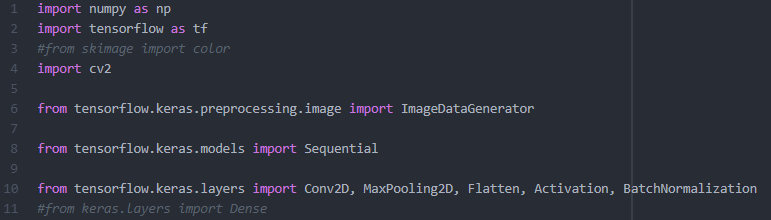
\includegraphics[width=1.0\textwidth]{bsp.png}
	\caption{Hier kann man dann auch noch etwas dazu schreiben}
	\label{bsp}
\end{figure}
As previously mentioned we re-implemented the main ideas from the paper by Zhang et al. (2016). This was done with two approaches, which are going to be explained in more detail in this chapter. In both approaches the ImageNet2012 dataset was used. Firstly, we implemented the model structure as described in the paper (see figure 1) and trained the model with the color layers of the input images as the target. Secondly, we translated the colorization task to a classification problem and trained the same model structure with the altered problem representation.
\begin{figure}[ht]
	\centering
	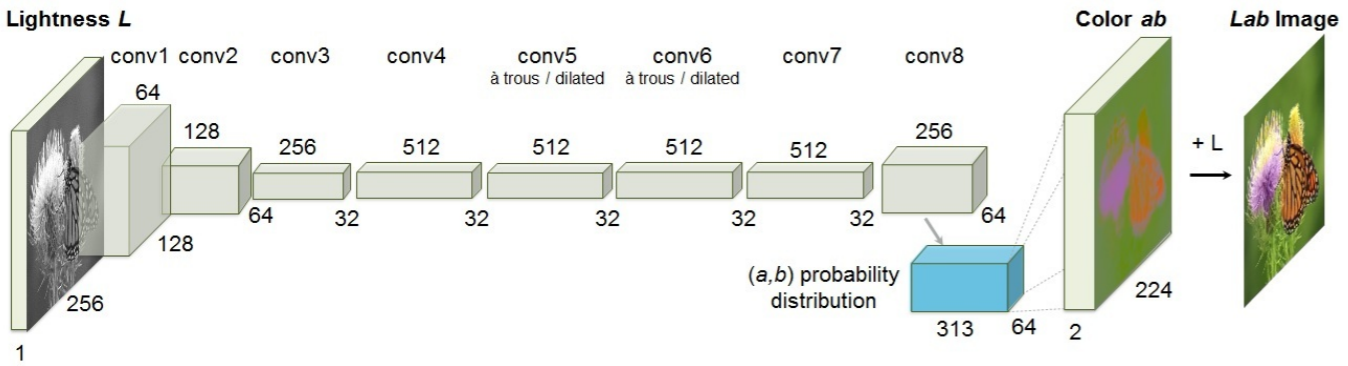
\includegraphics[width=1.0\textwidth]{layer.png}
	\caption{The network architecture of Zhang et al. (2016). }
	\label{fig1}
\end{figure}
- theoretical basis:\\

\subsection{The Data}
To train our model we used images from the ImageNet2012 challenge, which were also used in the paper by Zhang et al. and which were available to us through the university server. As we were working with a large amount of data in each batch, it would have been impossible to load the whole dataset at once, hence we used a data generator to load the input and target images successively for each batch. Although there are inbuilt data generators available from keras that allow for some means of data augmentation, we built our costum generator to ensure the functionality we were aiming at. The generator takes the batch size and a list which contains the paths to the images that should be used. Besides the functionalities that one would expect, like shuffling after the whole training set has been seen, the generator further creates the input and target arrays as described in the following.
First, the images are loaded and resized to a uniform shape of (224, 224, 3), which corresponds to the height, the width and the number of the color channels, respectively. Then the images are transformed from BGR to LAB color space. The luminance layer (L layer) which displays most of the structure, is separated from the other two and used as the input for our model.  The remaining two layers (ab layers) encode the color information of the images and are used as the target of the model in the first approach. In the second approach, these first steps remain the same, but additionally the target arrays are transformed to match a classification task.\\
This is done in three main steps. The first step is to discretize the continuous color space and reduce the number of possible colors by quantizing the a and b color ranges into 11 bins. This yields a total of 121 possible colors by combining the a and b layers. In the second step, the a and b layers are combined into a single layer, which keeps the same height and width dimensions as before. This means the color information of each pixel is now encoded in a single number rather than two. Cantor pairing is used to generate a unique and deterministic number from the two a and b values of each pixel. As cantor pairing is reversible, one can easily translate the pairing result back to the original color values with no loss of information. Now that there is a single value for each pixel that encodes its color, the third and last step is to translate this value into a one-hot encoding. With the help of a dictionary, the cantor values are translated to the numbers from 0 to 120. These numbers then serve as the index in the one hot encoding. Hence, color values that were previously represented in two values (a and b color channels) are now encoded by the index within the one-hot encoding. The target array has a shape of (224, 224, 121) and at each pixel position lies a one hot vector.\\
- loading large amount of data\\
\url{https://machinelearningmastery.com/how-to-load-large-datasets-from-directories-for-deep-learning-with-keras/}\\
das ist \citep{Brownlee.2019}
\subsection{The Model}
The model structure is strongly inspired by the original implementation by Zhang et al. Only minor changes occur, mostly due to the translation from caffe to keras. The model consists of eight blocks of two or three repeated convolution and relu activation layers followed by a batch normalization. There are no pooling layers in the model, as changes  in  resolution  are  achieved  through  spatial  downsampling  or  upsampling between the convolution blocks. A transpose convolutional layer is used to inverse the convolution and upsample the output back to the correct size.\\
In the first approach, a stochastic gradient descent optimizer (SGD optimizer) with a learning rate of 0.001 and a momentum of 0.9 is used, which is inspired by the original paper. Further, this approach uses mean squared error as the loss function. In the second approach, the softmax activation function is used in the last layer to prepare the model's output for the categorical crossentropy loss that is used in this approach. Besides, both SGD and Adam optimizer are tested. In both approaches, kernel weights are initialized with the glorot uniform initializer which draws samples from a uniform distribution depending on the number of input and output units of the corresponding weight tensor. Biases are initialized as zeros.\\


- image preprocessing documentation\\
\url{https://keras.io/preprocessing/image/#imagedatagenerator-class}\\
- preprocessing via ImageDataGenerator() from keras.prepeocessing.image\\
- takes in traindata, validation data and test data\\
- featurewise-center and featurewise std\\
- classmode: none -> is for predictions\\

\subsection{Modelstructure}
- besser hier layer und loss-function
\subsection{Layer}
- built the same layers aas Zhang et al, but no probability distribution\\
-networkstructure and design\\

\subsection{Loss-Function}
- the original loss-function\\
- we tried what loss function?\\
\section{Visualization and discussion of your results.}
oder lieber bilder als screenshot einfügen?\\
\subsection{Training}
The models were trained on the grid of the institute of cognitive science at Osnabrueck University. A helper script was written that distributed several grid jobs on different computers in order to experiment with the hyperparameters such as the learning rate and the batch size. Through this script, one can easily change these parameters as well as select the data set and the environment and switch between the training mode and the prediction mode. The models were trained with 2000 images and batch sizes of 10 or 20 images. The learning rate varied from 0.1 to 0.001.

\subsection{Testing}
To evaluate the goodness of our two approaches, colors for unseen test images are predicted and evaluated via visual inspection. When the script is started in prediction mode, the model is not trained, but the weights from the corresponding training process are loaded. The model then predicts the most plausible colors for the L layers of the input images.
In the first approach, the model's output can be interpreted as the ab layers. That means the output can be combined with the input (L layer) and displayed as an image straight away.
For the second approach, three decoding steps are necessary before yielding human-readable images. Firstly, the output of the softmax layer is decoded to find the index of the most likely color value. Secondly, this index is translated to the cantor pairing value it represents with the help of a dictionary. And thirdly, the cantor pairing value is transformed back to the a and b values it is constituted of. These a and b layers can finally be combined with the L layer to display the predicted image in LAB color space.

\subsection{Conclusion and Future Work}
- vergleich ziehen zu Zhang\\
\newpage
\thispagestyle{empty}
\section{Literature}
\label{Lit}
\bibliographystyle{apa}
\renewcommand{\bibsection}{}

\bibliography{lit}
	
\end{document}
